\documentclass{article}
\usepackage[table]{xcolor}
\usepackage{titlepic}
\usepackage{hyperref}
\usepackage{amsmath}
\usepackage{enumitem}% http://ctan.org/pkg/enumerate
\usepackage{rotating} 
\usepackage{float}
\usepackage{multirow}
\usepackage[margin=0.5in]{geometry}
\usepackage{titling}
\usepackage{capt-of}
\usepackage{siunitx}
%\usepackage{arydshln}
\usepackage{longtable}
\usepackage{xcolor}
\usepackage{colortbl}
%\usepackage[justification=centering]{caption}
%\usepackage{caption}
\sisetup{group-separator = {,}, group-minimum-digits = 4}
\definecolor{CSONavy}{HTML}{405381}
\hypersetup{
    colorlinks,
    linkcolor={black!50!black},
    citecolor={blue!50!black},
    urlcolor={blue!80!black}
}
\urlstyle{same}
%\nocite{*}
%\setlength{\droptitle}{-4.5em}

%\titlepic{
\includegraphics{../figures/CSO_Logo.png}}
\title{Electoral Division Health Profile - Curraclone, Laois}
%\date{\vspace{-5ex}}
\date{Census 2022}
\author{CSO, Ireland  (\url{http://www.cso.ie)}}

\newcolumntype{T}{>{\raggedleft\arraybackslash}m{1.7cm}}
\newcolumntype{O}{>{\centering\arraybackslash}m{3.4cm}}
\newcolumntype{M}{>{\raggedleft\arraybackslash}m{3cm}}
\newcolumntype{A}{>{\raggedright\arraybackslash}m{9.5cm}}
\newcolumntype{S}{>{\raggedleft\arraybackslash}m{1.4cm}}
\newcolumntype{K}{>{\raggedright\arraybackslash}m{7.5cm}}

\usepackage{Sweave}
\begin{document}
\Sconcordance{concordance:25-curraclone-laois-ac-laois-county-council.tex:HealthProfileTemplate.Rnw:1 44 1 1 0 845 1}

%
\includegraphics{../figures/CSO_Logo.png}
%\begin{minipage}{\linewidth}

\begin{figure}
	\centering

\includegraphics[width =75mm]{../figures/CSO_Logo.png}
\end{figure}

\begin{figure}[h]
	\centering
	\setlength{\fboxsep}{1pt}
	\fbox{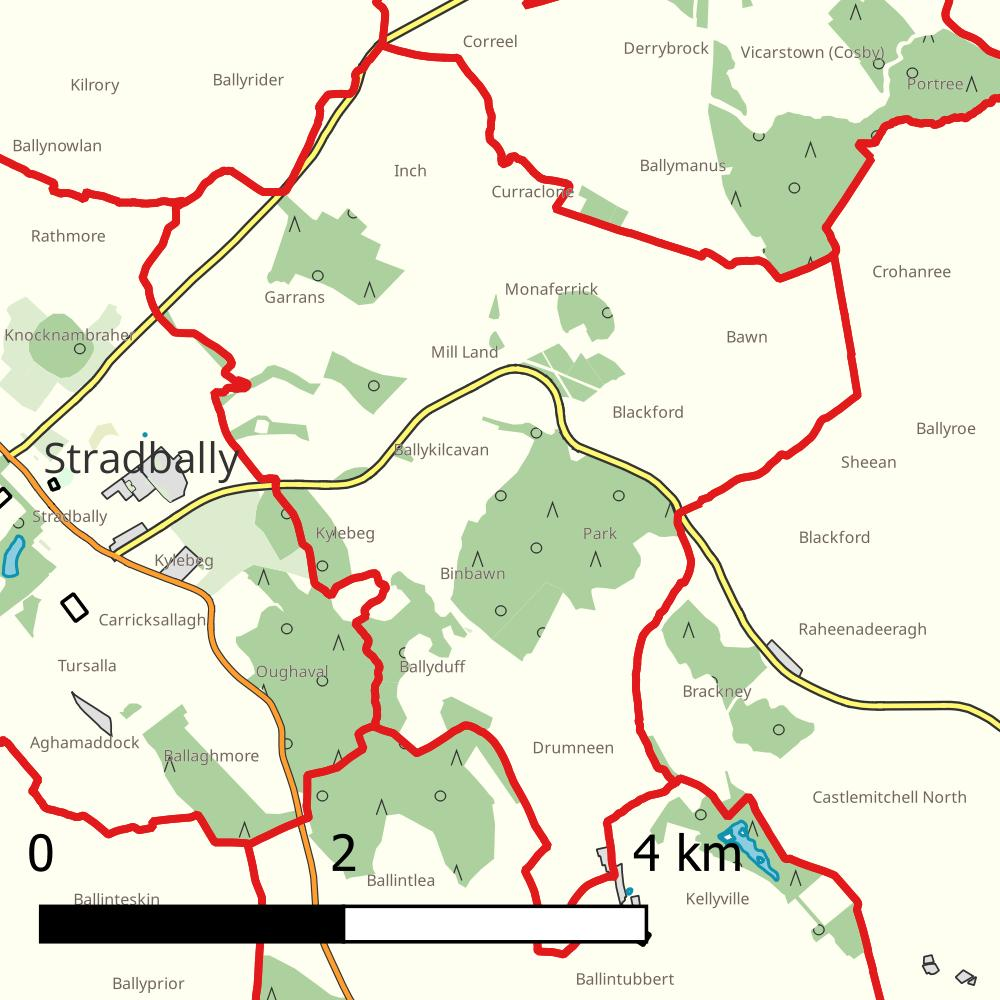
\includegraphics[width = 140mm]{../inputs/exportededmaps/2ae19629-16b5-13a3-e055-000000000001.jpg}}
	\caption{\normalsize Boundary Map for Curraclone, Laois Electoral Division (Sources: OSI, Ireland; OpenStreetMap). Map style by Champs-Libres Coop., distributed under CC BY-SA.}
	\label{fig:2ae19629-1a6a-13a3-e055-000000000001}
	\end{figure}
	{\let\newpage\relax\maketitle}
	     \begin{center}
         \emph{Profile generated on 21/10/2024}
     \end{center}
     	     \begin{center}
        \emph{Note: This is the first time this profile has been compiled. While efforts have been made to ensure that everything in this document is correct, it is possible that there may be some errors. Please email tomas.kelly@cso.ie if you observe any errors or inconsistencies with other CSO data.}
     \end{center}
    %\maketitle[h]
  \pagebreak
    	    \tableofcontents
%\end{minipage}

\pagebreak


\section{Key Points}

\begin{itemize}

\item Curraclone, Laois covers a total \textbf{area} of  \textbf{12.8 square kilometers} and has a \textbf{population density of 21.1} persons per square kilometer. The population density of Ireland as a whole is  73.3. 

\item The \textbf{Age Dependency Ratio} of this Electoral Division (ED) is  \textbf{58.2}. This compares to 53.2 nationally. The Age Dependency Ratio is the amount of people outside of working age (0-14 and 65+) per 100 people of working age (15-64). 

\item Curraclone, Laois has a total of \textbf{269} \textbf{persons} and  \textbf{75} \textbf{families} living in private households.

\item There are a total of \textbf{59 persons aged 0-14} in this ED and \textbf{40 persons aged over 65.} 

\item There are a total of \textbf{59} persons \textbf{living with a disability} in this ED, representing \textbf{21.9 percent} of the population. This compares with  21.5 percent nationally

\item \textbf{2} people in this ED have \textbf{bad or very bad general health}. This represents \textbf{0.7 percent} of the population. 1.7 percent of the population have bad or very bad general health nationally. 

\item There are a total of \textbf{18 carers} in this ED, representing \textbf{6.7 percent} of the population. This compares with 5.8 percent of the population that are carers nationally. 

\item \textbf{11.5 percent} of this ED \textbf{smoke tobacco products}. 13.1 percent of people nationally smoke tobacco products

\item There are \textbf{2 short term unemployed} and \textbf{0 long term unemployed} people in this ED. These represent 1.0 and 0.0 percent of the population respectively.

\item  \textbf{3.0 percent} of the population of Curraclone, Laois are \textbf{unskilled}. 3.1 percent of people in the state are unskilled.

\item \textbf{28 percent} of those aged 15+ in this ED have a \textbf{highest level of education of lower secondary or lower}. This compares with 23 percent nationally. 

\item \textbf{11.1 percent} of families with children in this ED have \textbf{lone parents}. This stands at 24.8 nationally.

\item \textbf{6 percent} of this ED were \textbf{born outside Ireland} (20 percent nationally).

\item \textbf{Households rented from a Local Authority} comprise \textbf{0.0 percent} of households in this ED.This stands at 8.3 percent nationally

\end{itemize}

\pagebreak

\section{Population} 
\label{sect:Pop}

\begin{figure}[h]
	\centering
	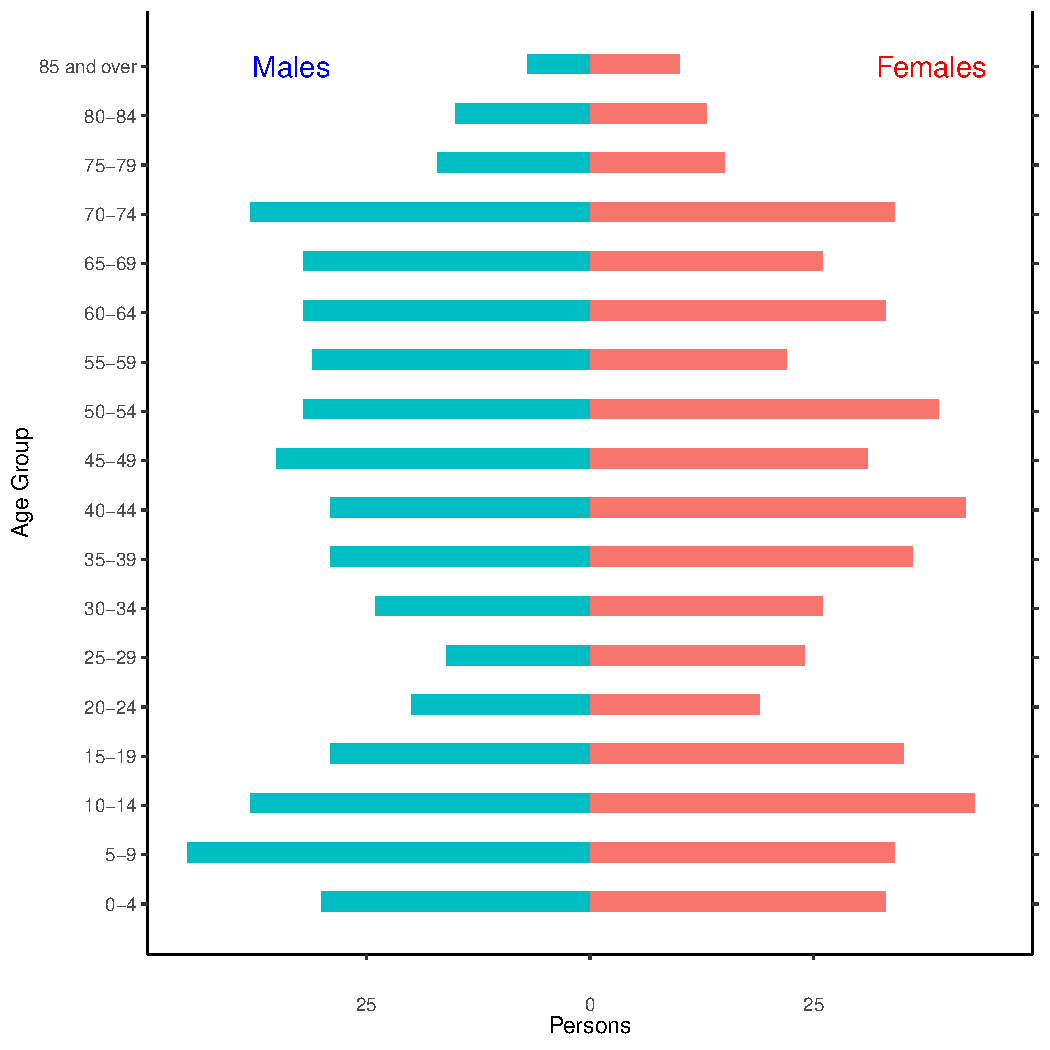
\includegraphics[width = 100mm]{../figures/PyramidPlot.pdf}
	\caption{Persons by Age Group and Gender for Curraclone, Laois; Administrative County and State; Census 2022.}
	\label{fig:2ae19629-1a6a-13a3-e055-000000000001}
	\end{figure}

\begin{table}[!h]
\centering
\begin{tabular}{lSSSSSSSSS}
  \hline
 \textbf{Age} & \multicolumn{2}{c}{\textbf{Females}} & \multicolumn{2}{c}{\textbf{Males }} & \multicolumn{4}{c}{\textbf{Both Sexes}}  \\ 
\cline{6-9}\\
 & \emph{\textbf{Persons}} & \emph{\textbf{\%}} & \emph{\textbf{Persons}} & \emph{\textbf{\%}} & \emph{\textbf{Persons}} & \emph{\textbf{\% (ED)}} & \emph{\textbf{\% (AC)}}& \emph{\textbf{\% (State)}}\\
  \hline
  0-14   & 29 &  22.8 & 30 & 21.1 & 59 &21.9 & 22.2 & 19.7 \\
  15-64  & 77 & 60.6 & 93 & 65.5 & 170&63.2 & 64.8 &65.3\\
  65+ & 21 & 16.5 & 19 & 13.4 &40 &14.9 & 13.0 & 15.1 \\
 \hline
  Age 0-4  & 9& 7.1& 11 & 7.7& 20 & 7.4 & 6.2& 5.7 \\
  
  Age 5-9  & 10& 7.9& 10 & 7.0& 20 & 7.4 & 7.5& 6.7 \\

  Age 10-14  & 10& 7.9& 9 & 6.3& 19 & 7.1 & 8.5& 7.3 \\

  Age 15-19  & 4& 3.1& 18 & 12.7& 22 & 8.2 & 7.2& 6.6 \\

  Age 20-24  & 7& 5.5& 5 & 3.5& 12 & 4.5 & 5.4& 6.0 \\

  Age 25-29  & 5& 3.9& 8 & 5.6& 13 & 4.8 & 4.8& 5.7 \\

  Age 30-34  & 5& 3.9& 6 & 4.2& 11 & 4.1 & 5.9& 6.5 \\

  Age 35-39  & 9& 7.1& 9 & 6.3& 18 & 6.7 & 8.0& 7.4 \\

  Age 40-44  & 6& 4.7& 6 & 4.2& 12 & 4.5 & 8.4& 8.0 \\
  
    Age 45-49  & 16& 12.6& 12 & 8.5& 28 & 10.4 & 7.4& 7.3 \\
  
    Age 50-54  & 11& 8.7& 15 & 10.6& 26 & 9.7 & 6.8& 6.6 \\
  
    Age 55-59  & 7& 5.5& 5 & 3.5& 12 & 4.5 & 5.8& 6.0 \\
  
    Age 60-64  & 7& 5.5& 9 & 6.3& 16 & 5.9 & 5.1& 5.3 \\
  
    Age 65-69  & 5& 3.9& 4 & 2.8& 9 & 3.3 & 4.3& 4.6 \\
  
    Age 70-74  & 7& 5.5& 2 & 1.4& 9 & 3.3 & 3.4& 3.9 \\
  
    Age 75-79  & 4& 3.1& 10 & 7.0& 14 & 5.2 & 2.6& 3.0 \\
  
    Age 80-84  & 3& 2.4& 2 & 1.4& 5 & 1.9 & 1.5& 1.9\\
  
    Age 85 and over  & 2& 1.6& 1 & 0.7& 3 & 1.1 & 1.2& 1.6 \\
  
    All Ages  & 127& 100.0& 142 & 100.0& 269 & 100.0 & 100.0& 100.0 \\
      \hline 
    \multicolumn{4}{l}{\href{https://data.cso.ie/table/SAP2022T1T1AED}{https://data.cso.ie/table/SAP2022T1T1AED}} & & &
\end{tabular}
\caption{Population Breakdown by Age and Sex for Curraclone, Laois; Census 2022. Percentage breakdowns for Administrative County (AC) and State are provided for comparison purposes.}
\end{table}

\pagebreak

\section{Disability}\label{sect:Disability}
\begin{figure}[h]
	\centering
	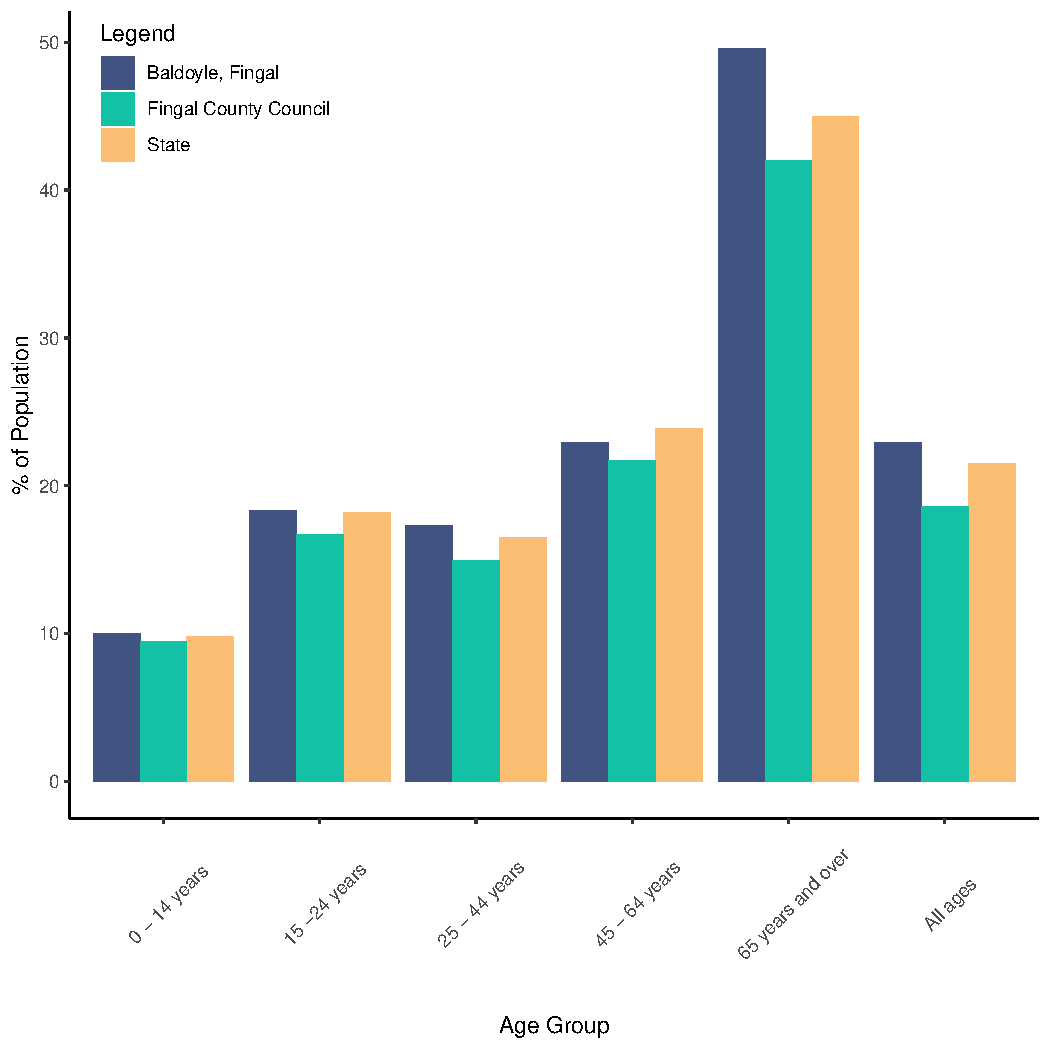
\includegraphics[width = 130mm]{../figures/DisED.pdf}
	\caption{Percentage of Population with any Disability by Age Group for Curraclone, Laois; Administrative County and State; Census 2022.}
	\label{fig:2ae19629-1a6a-13a3-e055-000000000001}
	\end{figure}


\begin{table}[!h]
\centering
\begin{tabular}{lTTTTT}
  \hline
 & \multicolumn{3}{c}{\textbf{Curraclone, Laois}} & \textbf{Laois County Council} & \textbf{State}\\ 
 \cline{2-4} \\
  \textbf{Age Group} & \textbf{Population} & \multicolumn{4}{c}{\textbf{With any Disability}} \\
 \cline{3-6}\\
& \emph{\textbf{Persons}} & \emph{\textbf{Persons}} & \emph{\textbf{\%}} & \emph{\textbf{\%}} & \emph{\textbf{\%}}\\
  \hline
  0-14  & 59& 6 & 10.2 & 11.3 & 9.8 \\
15-24  & 34& 6 & 17.6 &18.2 & 18.2 \\ 
25-44  & 54& 12 & 22.2 &17.4& 16.5 \\ 
45-64  & 82& 20 & 24.4 &25.7 &23.9 \\ 
65 years and over  & 40& 15 & 37.5 &45.3& 45.0 \\ 
All Ages  & 269& 59 & 21.9 &21.9 &21.5 \\ 
   \hline
       \multicolumn{4}{l}{\href{https://data.cso.ie/table/F4004}{https://data.cso.ie/table/F4004}} & 
\end{tabular}
\caption{Population with any Disability by Age Group for Curraclone, Laois; Census 2022. Percentage breakdowns for Administrative County and State are provided for comparison purposes.}
\end{table}

\pagebreak

\section{General Health}\label{sect:GenHealth}

\begin{figure}[h]
	\centering
	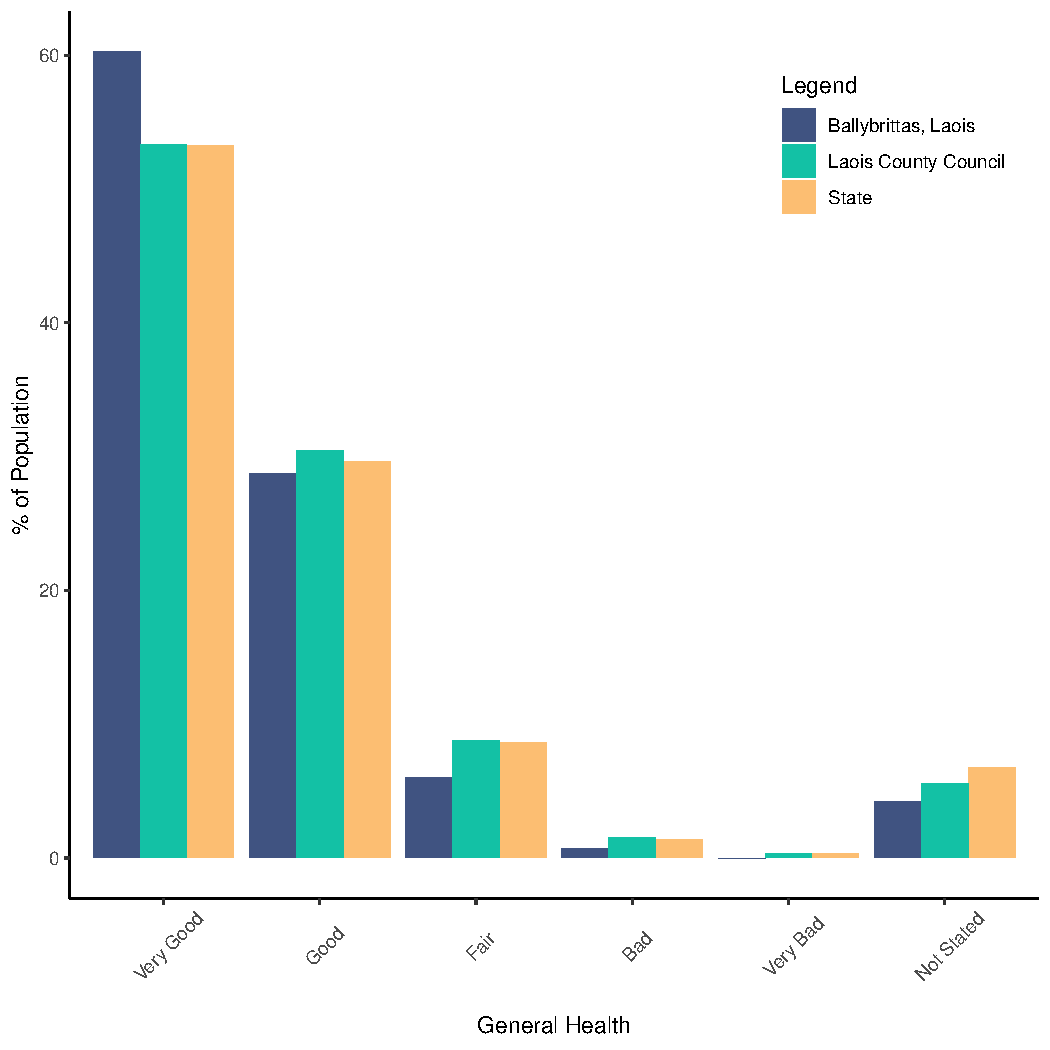
\includegraphics[width = 150mm]{../figures/GenED.pdf}
	\caption{Population Breakdown (\%) by General Health for Curraclone, Laois; Administrative County and State;  Census 2022.}
	\label{fig:2ae19629-1a6a-13a3-e055-000000000001}
	\end{figure}

\begin{table}[!h]
\centering
\begin{tabular}{lTTTTT}
  \hline
\textbf{General Health} & \multicolumn{2}{c}{\textbf{Curraclone, Laois}} & \textbf{Laois County Council} & \textbf{State}\\ 
 \cline{2-3} \\
 & \emph{\textbf{Persons}} & \emph{\textbf{\%}} & \emph{\textbf{\%}} & \emph{\textbf{\%}} \\
  \hline
Very Good& 165 &61.3 &53.3 &53.2 \\
Good& 69 &25.7 &30.4 &29.7\\
Fair& 27 &10.0 &8.8 &8.6\\
Bad& 2 &0.7 &1.5 &1.4\\
Very Bad& 0 &0.0 &0.3 &0.3\\
Not Stated& 6 &2.2 &5.6 &6.7\\
Total& 269 &100.0 &100.0 &100.0\\
   \hline
       \multicolumn{4}{l}{\href{https://data.cso.ie/table/SAP2022T12T3ED}{https://data.cso.ie/table/SAP2022T12T3ED}} & 
\end{tabular}
\caption{Population by General Health for Curraclone, Laois; Census 2022. Percentage breakdowns for Administrative County and State are also provided for comparison purposes.}
\end{table}
\pagebreak

\section{Carers}\label{sect:Carers}
\begin{figure}[H]
	\centering
	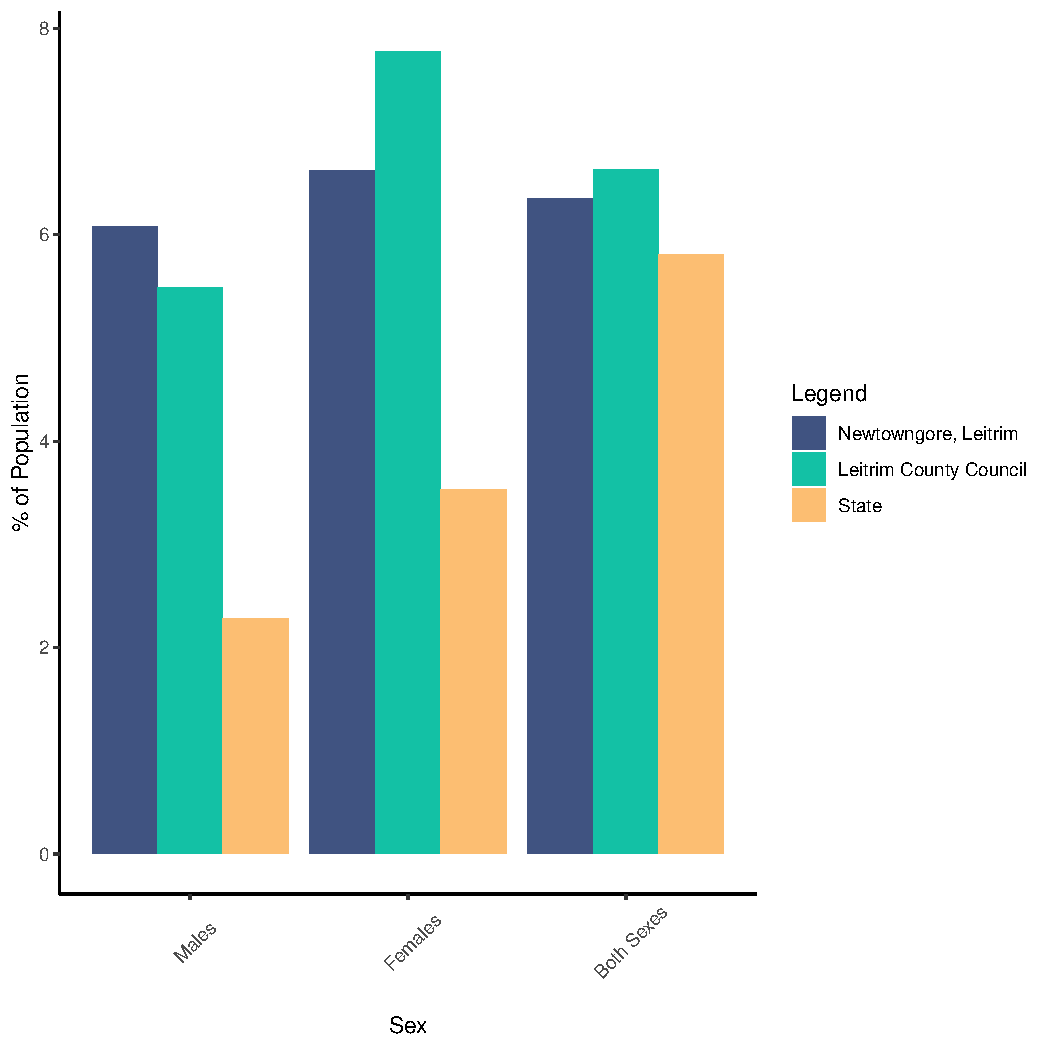
\includegraphics[width = 150mm]{../figures/CareED.pdf}
	\caption{Carers as a Percentage of the Population of Males/Females/Both Sexes for Curraclone, Laois; Administrative County and State; Census 2022.}
	\label{fig:2ae19629-1a6a-13a3-e055-000000000001}
	\end{figure}
	
	
\begin{table}[!h]	
\centering
	\begin{tabular}{lTTTTT}
  \hline
 & \multicolumn{3}{c}{\textbf{Curraclone, Laois}} & \textbf{Laois County Council} & \textbf{State}\\ 
 \cline{2-4} \\
  \textbf{Age Group} & \textbf{Population} & \multicolumn{4}{c}{\textbf{Carers}} \\
 \cline{3-6}\\
& \emph{\textbf{Persons}} & \emph{\textbf{Persons}} & \emph{\textbf{\%}} & \emph{\textbf{\%}} & \emph{\textbf{\%}}\\
  \hline
Males & 142 & 9  & 6.3  & 4.6 & 2.3 \\
Females & 127 & 9  & 7.1  & 7.4 & 3.5 \\
Both Sexes & 269 & 18  & 6.7  & 6.0 & 5.8 \\
     \hline
       \multicolumn{3}{l}{\href{https://data.cso.ie/table/SAP2022T12T2ED}{https://data.cso.ie/table/SAP2022T12T2ED}} 
\end{tabular}

\caption{Carers by Sex for Curraclone, Laois; Census 2022. Percentage Breakdowns for Administrative County and State are also provided for comparison purposes.}
\end{table} 

\pagebreak

\section{Volunteers}\label{sect:Volunteers}
\begin{figure}[H]
	\centering
	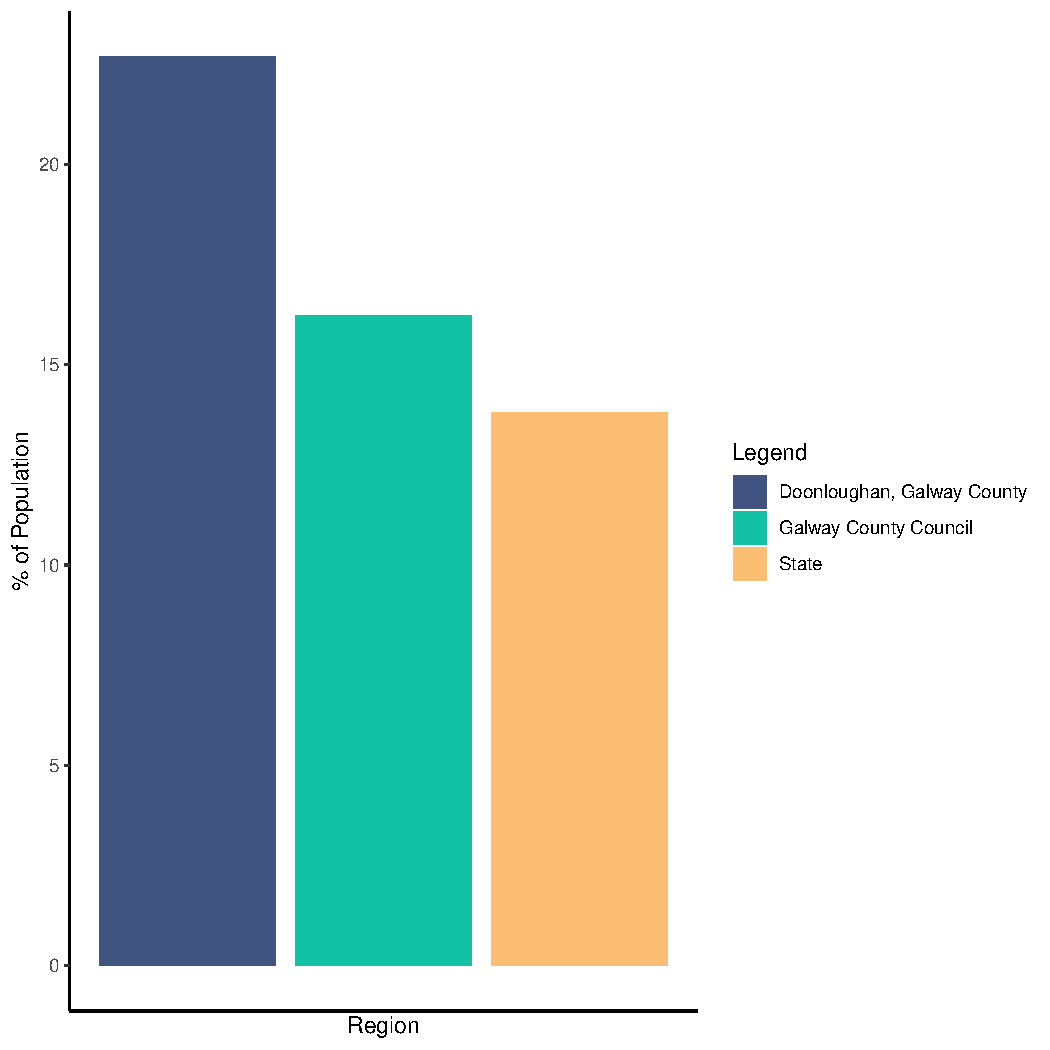
\includegraphics[width = 150mm]{../figures/VolunteerED.pdf}
	\caption{Volunteers as a Percentage of the Population for Curraclone, Laois; Administrative County and State; Census 2022.}
	\label{fig:2ae19629-1a6a-13a3-e055-000000000001}
	\end{figure}
	
	
\begin{table}[!h]	
\centering
	\begin{tabular}{lTTTTT}
  \hline
 & \multicolumn{3}{c}{\textbf{Curraclone, Laois}} & \textbf{Laois County Council} & \textbf{State}\\ 
 \cline{2-4} \\
  & \textbf{Population} & \multicolumn{4}{c}{\textbf{Volunteers}} \\
 \cline{3-6}\\
& \emph{\textbf{Persons}} & \emph{\textbf{Persons}} & \emph{\textbf{\%}} & \emph{\textbf{\%}} & \emph{\textbf{\%}}\\
  \hline
& 269 & 31  & 11.5  & 14.3 & 13.8 \\

     \hline
       \multicolumn{3}{l}{\href{https://data.cso.ie/table/SAP2022T7T1ED}} 
\end{tabular}

\caption{Volunteers for Curraclone, Laois; Census 2022. Percentage Breakdowns for Administrative County and State are also provided for comparison purposes.}
\end{table} 

\pagebreak

\section{Smoking}\label{sect:Smoking}
\begin{figure}[H]
	\centering
	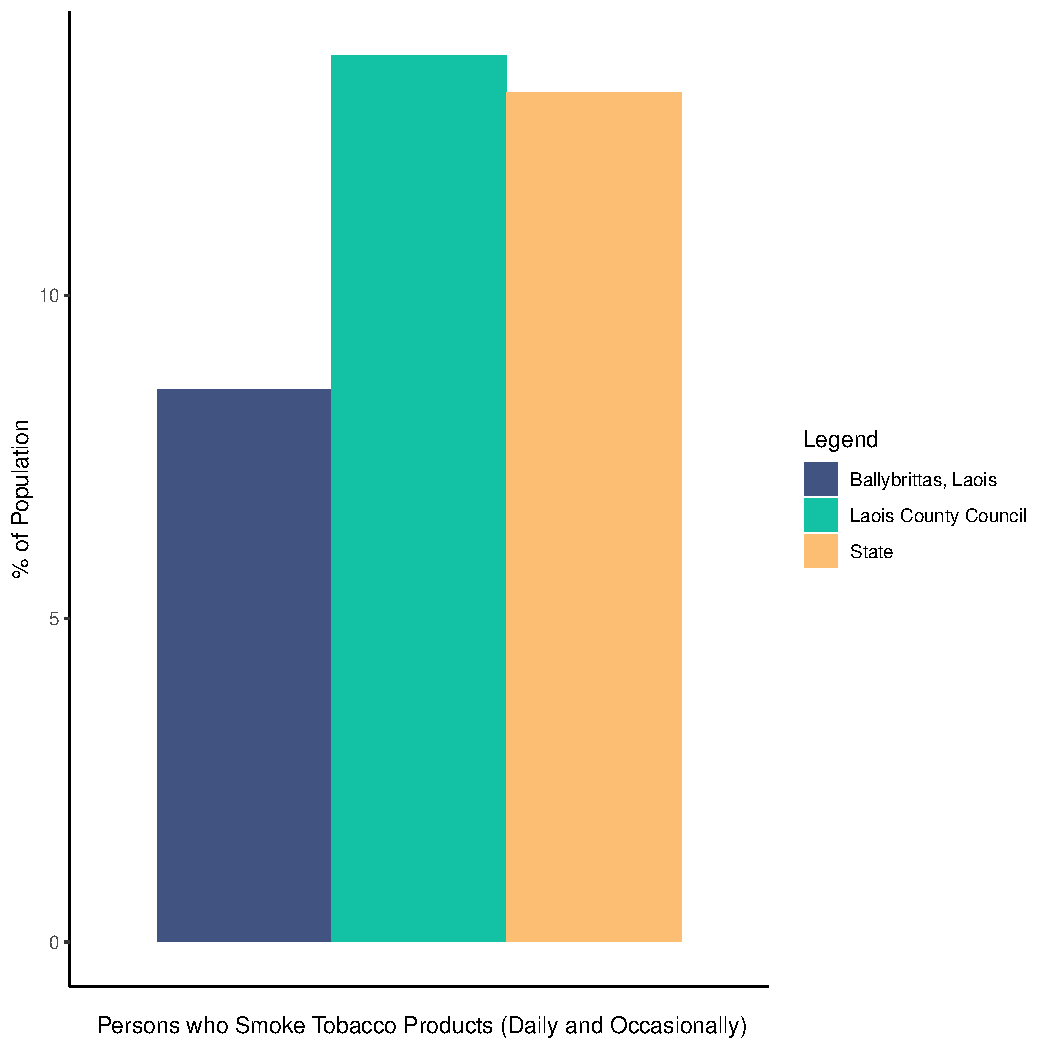
\includegraphics[width = 120mm]{../figures/SmokingED.pdf}
	\caption{Percentage of the Population who Smoke Tobacco Products (Daily and Occasionally) for Curraclone, Laois; Administrative County and State; Census 2022.}
	\label{fig:2ae19629-1a6a-13a3-e055-000000000001}
	\end{figure}
	
	
\begin{table}[!h]	
\centering
	\begin{tabular}{lTTTTT}
  \hline
  \textbf{Smoking Status} & \multicolumn{2}{c}{\textbf{Curraclone, Laois}} & \textbf{Laois County Council} & \textbf{State}\\ 
 \cline{2-3} \\
 & \emph{\textbf{Persons}} & \emph{\textbf{\%}} & \emph{\textbf{\%}} & \emph{\textbf{\%}} \\
  \hline
Smoke Tobacco Products (Daily and Occasionally)& 31 &11.5 &13.7 &13.1 \\
Don't Smoke Tobacco Products (Never and have given up)& 233 &86.6 &79.9 &79.4 \\
Smoking Status Not Stated& 5 &1.9 &6.4 &7.5 \\
All Persons & 269 & 100.0 & 100.0  & 100.0 \\
     \hline
      \multicolumn{3}{l}{\href{https://data.cso.ie/table/SAP2022T12T4ED}{https://data.cso.ie/table/SAP2022T12T4ED}} 
\end{tabular}

\caption{Smoking Status of Curraclone, Laois; Census 2022. Percentage breakdowns for Administrative County and State are also provided for comparison purposes.}
\end{table} 
    
  
\pagebreak
\section{Principal Economic Status}\label{sect:PES}
\begin{figure}[H]
	\centering
	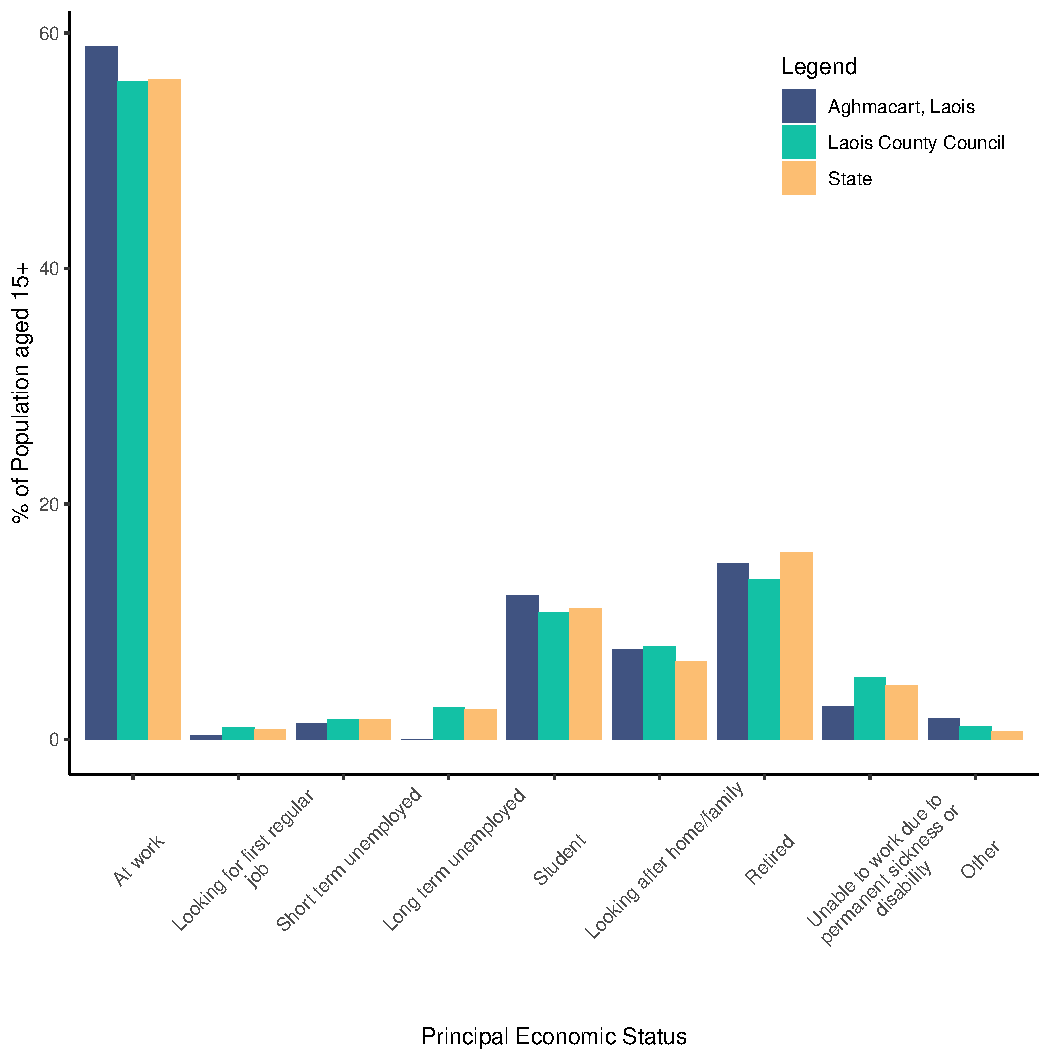
\includegraphics[width = 140mm]{../figures/PESED.pdf}
	\caption{Percentage of Population Aged 15+ by Principal Economic Status for Curraclone, Laois, Administrative County and State; Census 2022.}
	\label{fig:vbnv}
	\end{figure}

\begin{table}[h]	
\centering
		\begin{tabular}{lTTTTT}
  \hline
  \textbf{Principal Economic Status} & \multicolumn{2}{c}{\textbf{Curraclone, Laois}} & \textbf{Laois County...} & \textbf{State}\\ 
 \cline{2-3} \\
 & \emph{\textbf{Persons}} & \emph{\textbf{\%}} & \emph{\textbf{\%}} & \emph{\textbf{\%}} \\
  \hline
At Work & 117 &55.7 &55.9 &56.1 \\
Looking for first regular job & 0 &0.0 &1.0 &0.8 \\
Short term unemployed & 2 &1.0 &1.7 &1.7 \\
Long term unemployed & 0 &0.0 &2.8 &2.6 \\
Student & 25 &11.9 &10.8 &11.1 \\
 Looking after home/family & 17 &8.1 &7.9 &6.6 \\
Retired & 33 &15.7 &13.6 &15.9 \\
Unable to work due to permanent sickness or disability & 11 &5.2 &5.3 &4.6 \\
Other & 5 &2.4 &1.1 &0.7 \\
Total & 210 &100.0 &100.0 &100.0 \\
\hline
       \multicolumn{4}{l}{\href{https://data.cso.ie/table/SAP2022T8T1ED}{https://data.cso.ie/table/SAP2022T8T1ED}} &
\end{tabular}

\caption{Population aged 15+ by Principal Economic Status for Curraclone, Laois; Census 2022. Percentage breakdowns for Administrative County and State are also provided for comparison purposes.}
\end{table} 

\pagebreak

\section{Social Class}\label{sect:SC}
\begin{figure}[H]
	\centering
	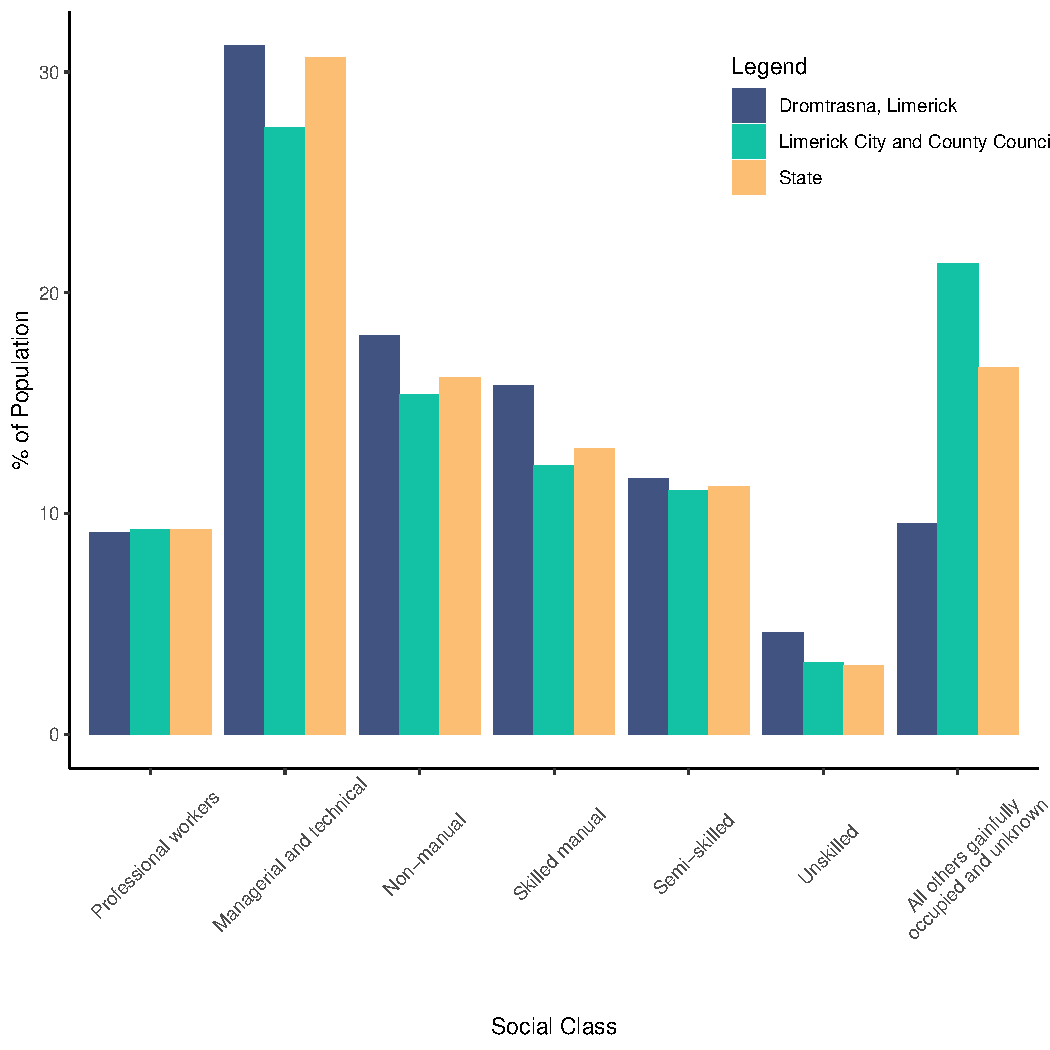
\includegraphics[width = 140mm]{../figures/SocialClassED.pdf}
	\caption{Percentage of Population Aged 15+ by Social Class for Curraclone, Laois, Administrative County and State; Census 2022.}
	\label{fig:vbnv}
	\end{figure}

\begin{table}[h]	
\centering
		\begin{tabular}{lTTTTT}
  \hline
  \textbf{Social Class} & \multicolumn{2}{c}{\textbf{Curraclone, Laois}} & \textbf{Laois County Council} & \textbf{State}\\ 
 \cline{2-3} \\
 & \emph{\textbf{Persons}} & \emph{\textbf{\%}} & \emph{\textbf{\%}} & \emph{\textbf{\%}} \\
  \hline
Professional workers & 35 & 13.0 & 6.6& 9.3\\
Managerial and technical & 86 & 32.0 & 29.7& 30.7\\
Non-manual & 69 & 25.7 & 17.8& 16.2\\
Skilled manual & 37 & 13.8 & 14.9& 12.9\\
Semi-skilled & 13 & 4.8 & 11.8& 11.2\\
Unskilled & 8 & 3.0 & 3.2& 3.1\\
All others gainfully occupied and unknown & 21 & 7.8 & 16.0& 16.6\\
Total & 269 & 100.0 & 100.0& 100.0\\
\hline
       \multicolumn{4}{l}{\href{https://data.cso.ie/table/SAP2022T9T1ED}{https://data.cso.ie/table/SAP2022T9T1ED}} &
\end{tabular}

\caption{Population aged 15+ by Social Class for Curraclone, Laois; Census 2022. Percentage breakdowns for Administrative County and State are also provided for comparison purposes.}
\end{table} 

\pagebreak
\section{Education}\label{sect:Edu}
\begin{figure}[H]
	\centering
	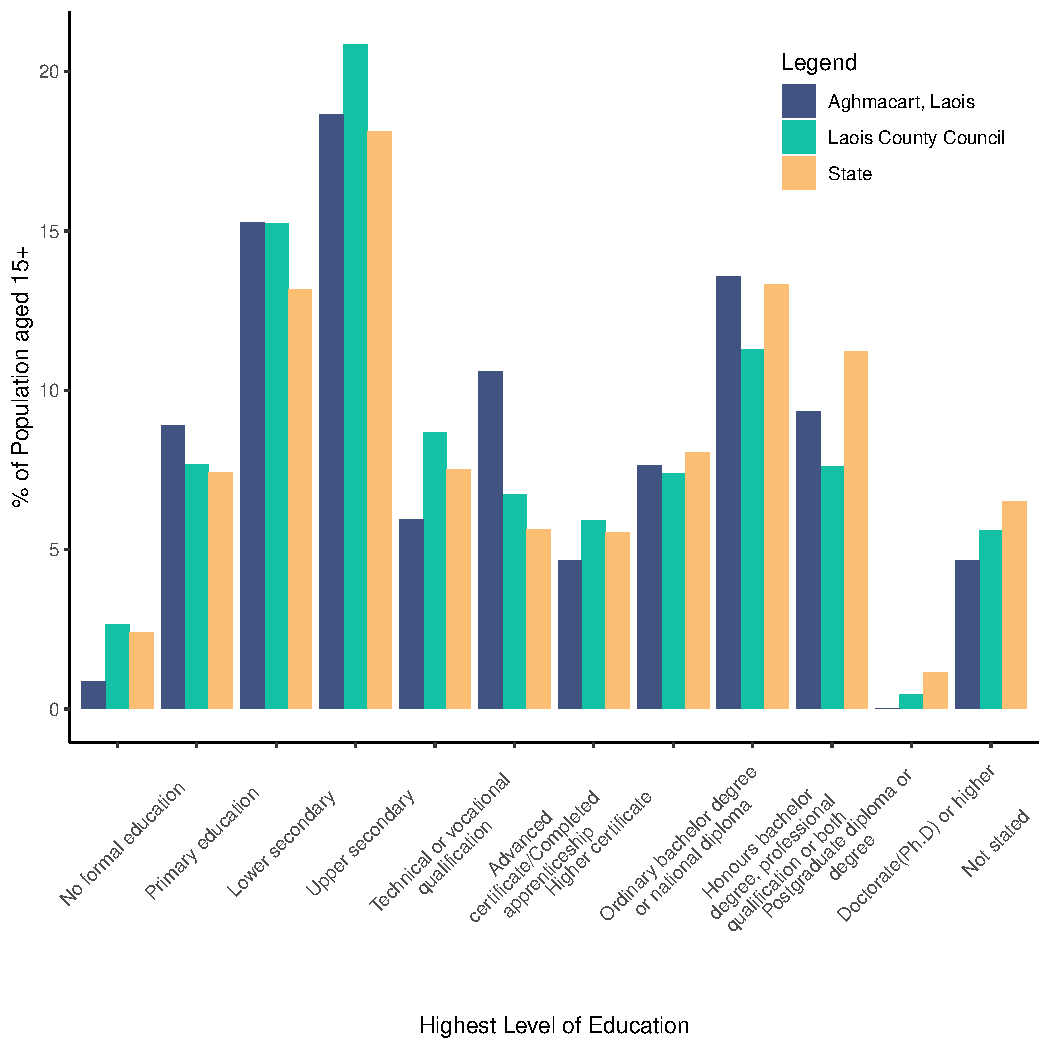
\includegraphics[width = 120mm]{../figures/EduED.pdf}
	\caption{Percentage of Population Aged 15+ by Highest Level of Education Completed for Curraclone, Laois; Administrative County and State; Census 2022.}
	\label{fig:vbnv}
	\end{figure}
\begin{table}[h]	
\centering
	\begin{tabular}{lTTTT}
  \hline
  \textbf{Highest Level of Education Completed} & \multicolumn{2}{c}{\textbf{Curraclone, Laois}} & \textbf{Laois County Council} & \textbf{State}\\ 
 \cline{2-3} \\
 & \emph{\textbf{Persons}} & \emph{\textbf{\%}} & \emph{\textbf{\%}} & \emph{\textbf{\%}} \\
  \hline
No formal education & 2 &1.1 &2.6 &2.4 \\
Primary education & 17 &9.3 &7.7 &7.4 \\
Lower secondary & 32 &17.6 &15.2 &13.2 \\
Upper secondary & 28 &15.4 &20.8 &18.1 \\
Technical or vocational qualification & 15 &8.2 &8.7 &7.5 \\
Advanced certificate/Completed apprenticeship & 16 &8.8 &6.7 &5.6 \\
Higher certificate & 12 &6.6 &5.9 &5.5 \\
Ordinary bachelor degree or national diploma & 12 &6.6 &7.4 &8.1 \\
Honours bachelor degree, professional qualification or both & 30 &16.5 &11.3 &13.3 \\
Postgraduate diploma or degree & 15 &8.2 &7.6 &11.2 \\
Doctorate(Ph.D) or higher & 2 &1.1 &0.4 &1.1 \\
Not stated & 1 &0.5 &5.6 &6.5 \\
Total & 182 &100.0 &100.0 &100.0 \\
   \hline
       \multicolumn{4}{l}{\href{https://data.cso.ie/table/SAP2022T10T4ED}{https://data.cso.ie/table/SAP2022T10T4ED}} &
\end{tabular}

\caption{Population aged 15+ by Highest Level of Education Completed for Curraclone, Laois; Census 2022. Percentage breakdowns for Administrative County and State are also provided for comparison purposes.}
\end{table} 
\pagebreak    
    
\section{Families}\label{sect:Fam}
\begin{figure}[H]
	\centering
	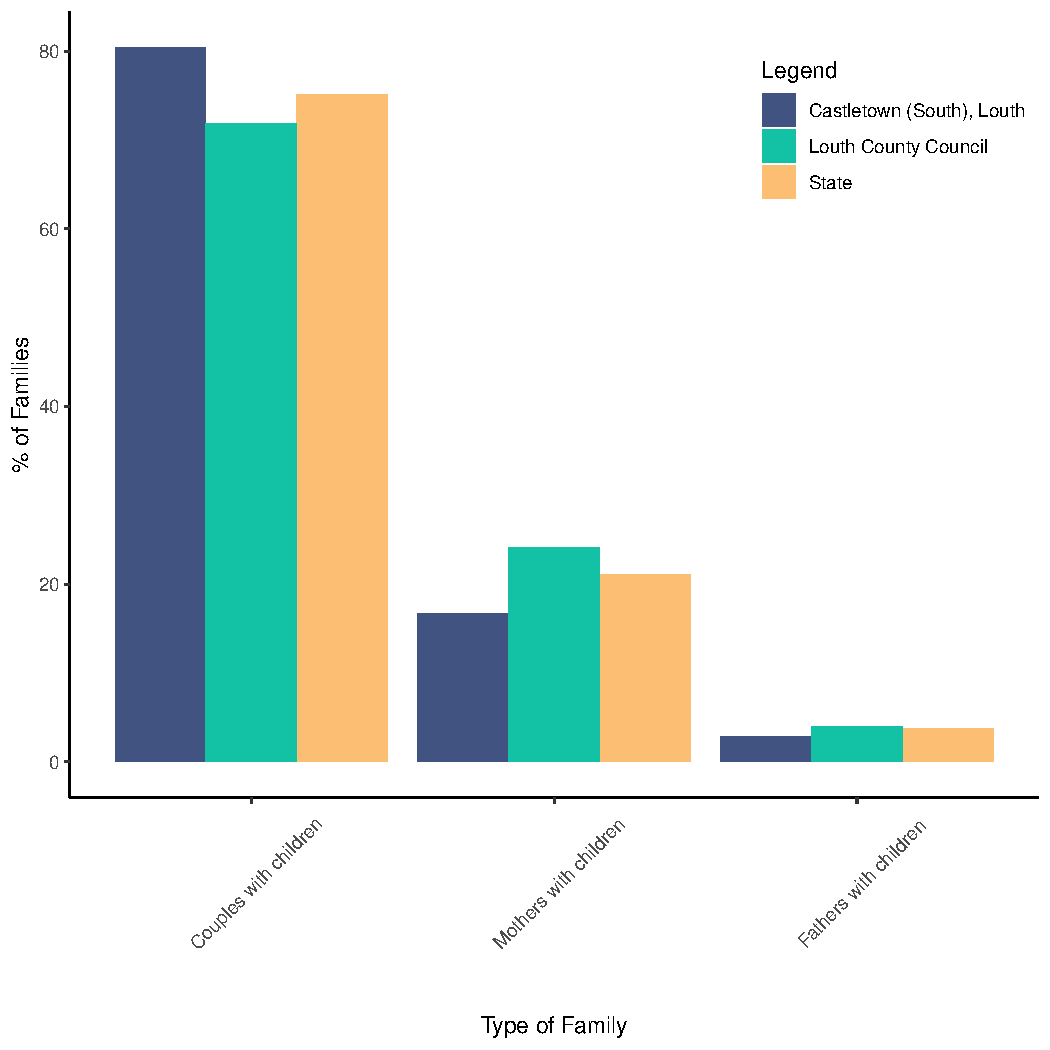
\includegraphics[width = 150mm]{../figures/FamED.pdf}
	\caption{Percentage of Families with Children by Family Type for Curraclone, Laois; Administrative County and State; Census 2022.}
	\label{fig:vbnv}
	\end{figure}
	
	
\begin{table}[h]	
\centering
\begin{tabular}{lTTTT}
  \hline
  \textbf{Type of Family} & \multicolumn{2}{c}{\textbf{Curraclone, Laois}} & \textbf{Laois County Council} & \textbf{State}\\ 
 \cline{2-3} \\
 & \emph{\textbf{Families}} & \emph{\textbf{\%}} & \emph{\textbf{\%}} & \emph{\textbf{\%}} \\
  \hline
Couples with Children & 48 &88.9 &76.8 &75.2 \\
Mothers with Children & 4 &7.4 &19.4 &21.1 \\
Fathers with Children & 2 &3.7 &3.8 &3.8 \\
All Families & 54 & 100.0 & 100.0  & 100.0 \\
  \hline
       \multicolumn{4}{l}{\href{https://data.cso.ie/table/SAP2022T4T3ED}{https://data.cso.ie/table/SAP2022T4T3ED}}  &
\end{tabular}

\caption{Families with Children by Family Type for Curraclone, Laois; 2022. Percentage breakdowns for Administrative County and State are also provided for comparison purposes.}
\end{table} 
\pagebreak

\section{Birthplace}\label{sect:Birth}
\begin{figure}[H]
	\centering
	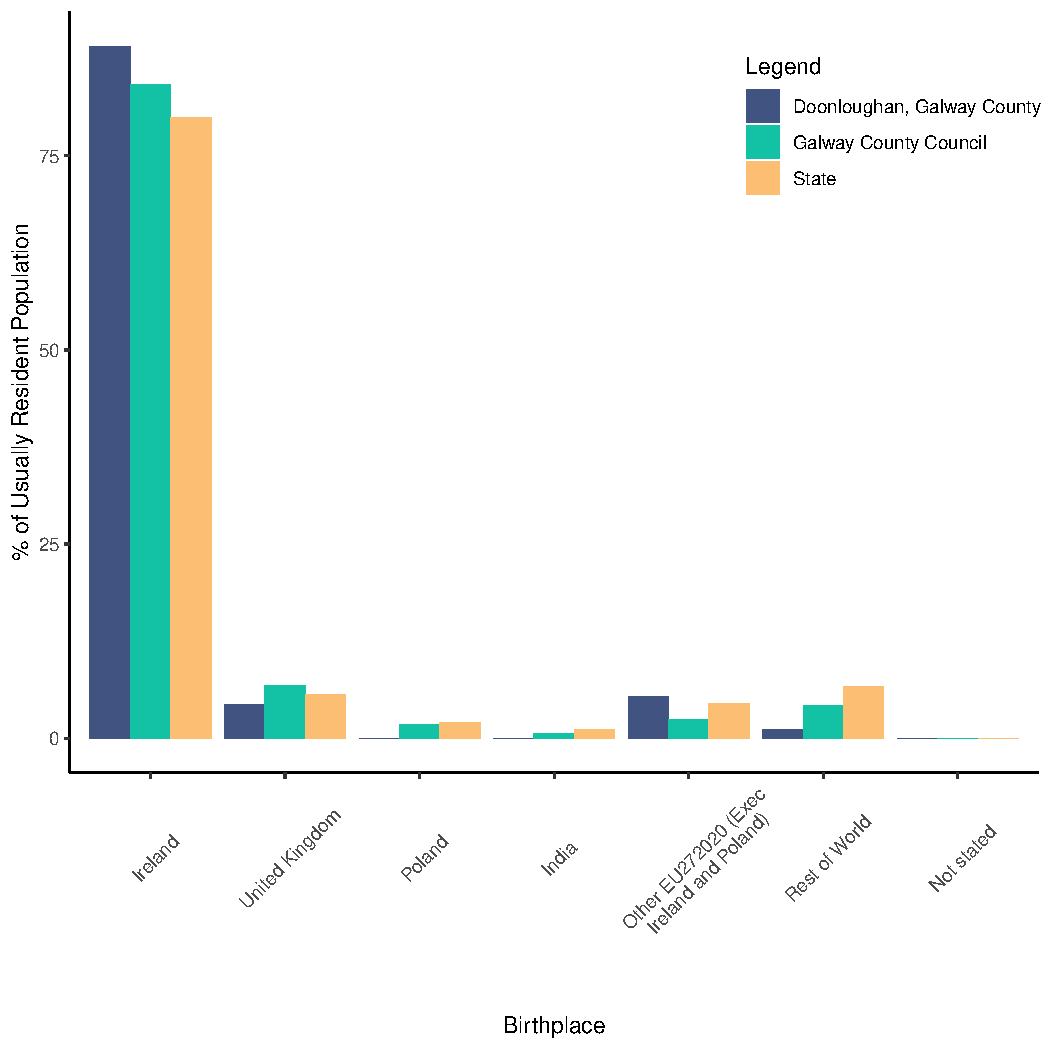
\includegraphics[width = 130mm]{../figures/BirthED.pdf}
	\caption{Percentage of Usually Resident Population by Birthplace for Curraclone, Laois; Administrative County and State; Census 2022.}
	\label{fig:vbnv}
	\end{figure}
	
	
\begin{table}[h]	
\centering
	\begin{tabular}{lTTTT}
  \hline
  \textbf{Birthplace} & \multicolumn{2}{c}{\textbf{Curraclone, Laois}} & \textbf{Laois County Council} & \textbf{State}\\ 
 \cline{2-3} \\
 & \emph{\textbf{Persons}} & \emph{\textbf{\%}} & \emph{\textbf{\%}} & \emph{\textbf{\%}} \\
  \hline
Ireland & 252 &94.0 &83.8 &80.0 \\
United Kingdom & 8 &3.0 &4.2 &5.7 \\
Poland & 0 &0.0 &2.8 &2.1 \\
India & 1 &0.4 &0.4 &1.1 \\
Other EU272020 (Exec Ireland and Poland) & 1 &0.4 &3.7 &4.4 \\
Rest of World & 6 &2.2 &5.0 &6.7 \\
Not stated & 0 &0.0 &0.0 &0.0 \\
Total & 268 &100.0 &100.0 &100.0 \\
  \hline
       \multicolumn{4}{l}{\href{https://data.cso.ie/table/SAP2022T2T1ED}{https://data.cso.ie/table/SAP2022T2T1ED}} &
\end{tabular}

\caption{Usually Resident Population By Birthplace for Curraclone, Laois, Census 2022. Percentage breakdowns for Administrative County and State are also provided for comparison purposes.}
\end{table} 
\pagebreak

\section{Households - Type of Occupancy}\label{sect:Households}
\begin{figure}[H]
	\centering
	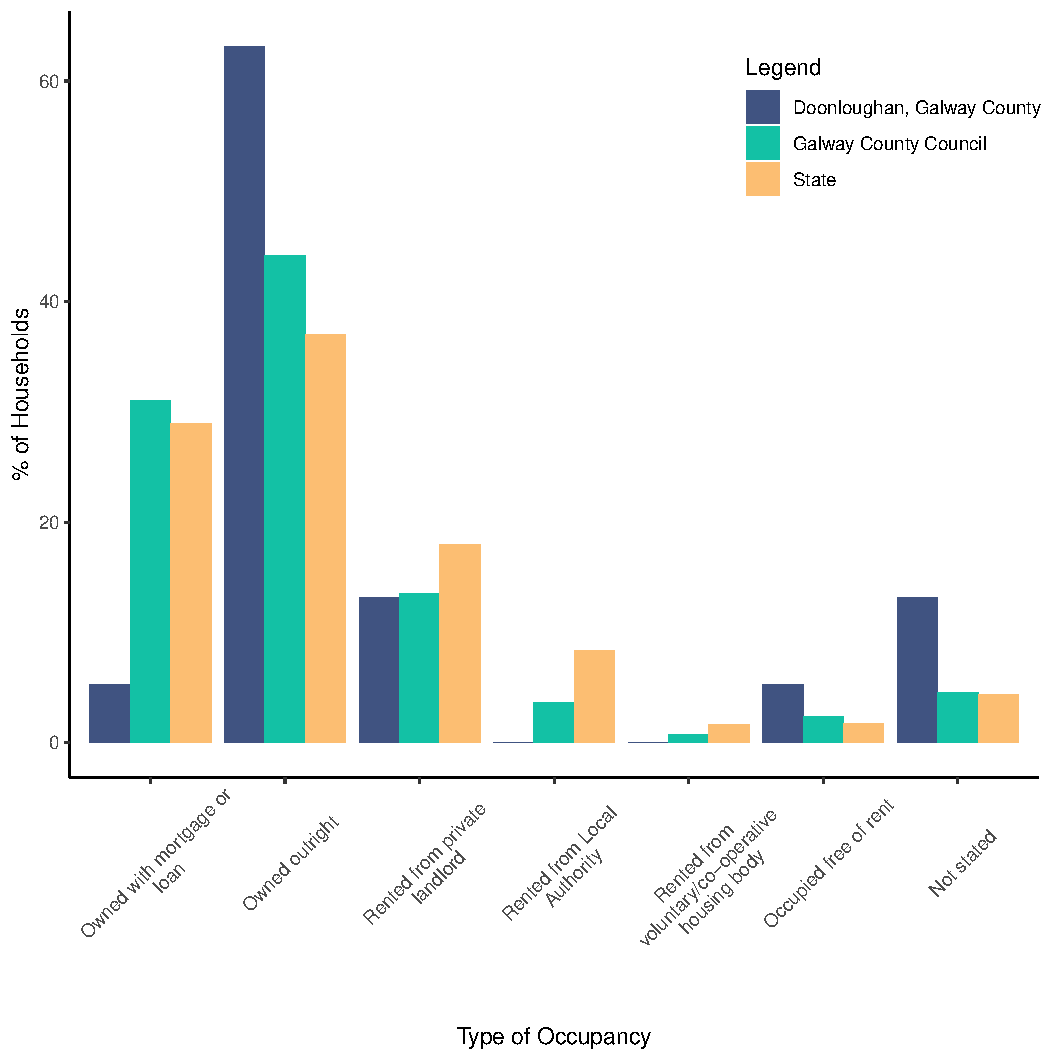
\includegraphics[width = 140mm]{../figures/HouseholdsED.pdf}
	\caption{Percentage of Households by Type of Occupancy for Curraclone, Laois, Administrative County and State; Census 2022.}
	\label{fig:vbnv}
	\end{figure}

\begin{table}[h]	
\centering
		\begin{tabular}{lTTTTT}
  \hline
  \textbf{Type of Occupancy} & \multicolumn{2}{c}{\textbf{Curraclone, Laois}} & \textbf{Laois County Council} & \textbf{State}\\ 
 \cline{2-3} \\
 & \emph{\textbf{Households}} & \emph{\textbf{\%}} & \emph{\textbf{\%}} & \emph{\textbf{\%}} \\
  \hline
Owned with mortgage or loan & 38 & 45.2 & 33.8 & 28.9 \\
Owned outright & 36 & 42.9 & 37.3 & 37.0 \\
Rented from private landlord & 4 & 4.8 & 12.9 & 18.0 \\
Rented from Local Authority & 0 & 0.0 & 8.5 & 8.3 \\
Rented from voluntary/co-operative housing body & 0 & 0.0 & 2.3 & 1.6 \\
Occupied free of rent & 2 & 2.4 & 1.8 & 1.7 \\
Not stated & 4 & 4.8 & 3.5 & 4.4 \\
Total & 84 & 100.0 & 100.0 & 100.0 \\
\hline
       \multicolumn{4}{l}{\href{https://data.cso.ie/table/SAP2022T6T3ED}{https://data.cso.ie/table/SAP2022T6T3ED}} &
\end{tabular}

\caption{Percentage of Households by Type of Occupancy for Curraclone, Laois; Census 2022. Percentage breakdowns for Administrative County and State are also provided for comparison purposes.}
\end{table} 

\pagebreak

\section{Transport}\label{sect:Trans}
\begin{figure}[H]
	\centering
	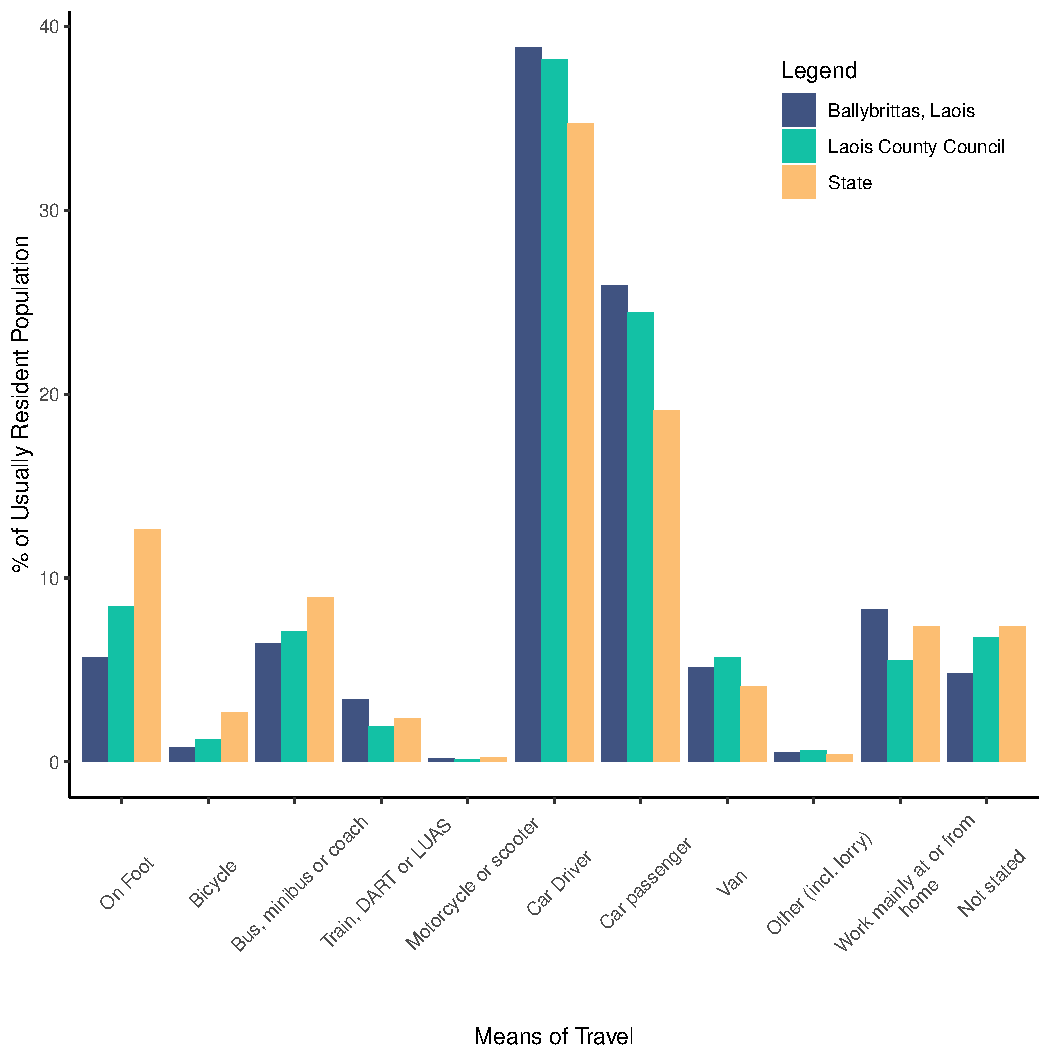
\includegraphics[width = 120mm]{../figures/TravelED.pdf}
	\caption{Percentage of Usually Resident Population by Means of Travel to Work, School, College or Childcare for Curraclone, Laois, Administrative County and State; Census 2022.}
	\label{fig:vbnv}
	\end{figure}

\begin{table}[h]	
\centering
		\begin{tabular}{lTTTTT}
  \hline
  \textbf{Means of travel} & \multicolumn{2}{c}{\textbf{Curraclone, Laois}} & \textbf{Laois County Council} & \textbf{State}\\ 
 \cline{2-3} \\
 & \emph{\textbf{Persons}} & \emph{\textbf{\%}} & \emph{\textbf{\%}} & \emph{\textbf{\%}} \\
 On Foot & 2 & 1.0 & 8.5 & 12.6 \\
Bicycle & 0 & 0.0 & 1.2 & 2.7 \\
Bus, minibus or coach & 14 & 7.1 & 7.1 & 9.0 \\
Train, DART or LUAS & 3 & 1.5 & 1.9 & 2.4 \\
Motorcycle or scooter & 0 & 0.0 & 0.1 & 0.3 \\
Car Driver & 87 & 44.4 & 38.2 & 34.7 \\
Car passenger & 62 & 31.6 & 24.4 & 19.1 \\
Van & 10 & 5.1 & 5.7 & 4.1 \\
Other (incl. lorry) & 0 & 0.0 & 0.6 & 0.4 \\
Work mainly at or from home & 13 & 6.6 & 5.5 & 7.4 \\
Not stated & 5 & 2.6 & 6.8 & 7.4 \\
Total & 196 & 100.0 & 100.0 & 100.0 \\
  \hline
       \multicolumn{4}{l}{\href{https://data.cso.ie/table/SAP2022T11T1ED}{https://data.cso.ie/table/SAP2022T11T1ED}} &
\end{tabular}

\caption{Percentage of Usually Resident Population by Means of Travel to Work, School, College or Childcare for Curraclone, Laois; Census 2022. Percentage breakdowns for Administrative County and State are also provided for comparison purposes.}
\end{table} 

\pagebreak

\section{Renewable Energy}\label{sect:RE}
\begin{figure}[H]
	\centering
	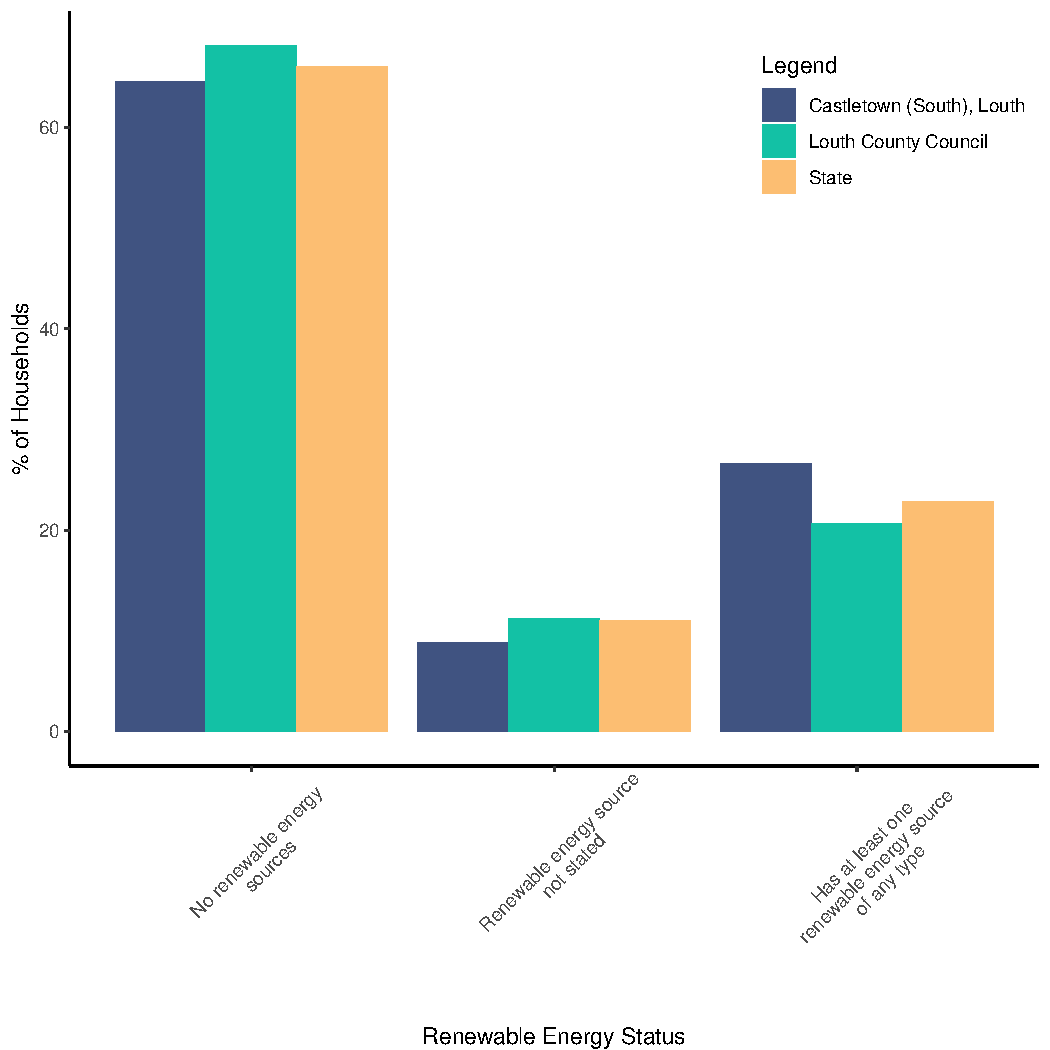
\includegraphics[width = 140mm]{../figures/RenewableEnergyED.pdf}
	\caption{Percentage of Households by Renewable Energy Source for Curraclone, Laois, Administrative County and State; Census 2022.}
	\label{fig:vbnv}
	\end{figure}

\begin{table}[h]	
\centering
		\begin{tabular}{lTTTTT}
  \hline
  \textbf{Renewable Energy Source} & \multicolumn{2}{c}{\textbf{Curraclone, Laois}} & \textbf{Laois County Council} & \textbf{State}\\ 
 \cline{2-3} \\
 & \emph{\textbf{Households}} & \emph{\textbf{\%}} & \emph{\textbf{\%}} & \emph{\textbf{\%}} \\
 No renewable energy sources & 36 & 42.9 & 63.2 & 66.1 \\
  Renewable energy source not stated & 7 & 8.3 & 9.6 & 11.0 \\
   Has at least one renewable energy source of any type & 41 & 48.8 & 27.1 & 22.9 \\
    All households & 84 & 100.0 & 100.0 & 100.0 \\
  \hline
       \multicolumn{4}{l}{\href{https://data.cso.ie/table/SAP2022T6T10ED}{https://data.cso.ie/table/SAP2022T6T10ED}} &
\end{tabular}

\caption{Percentage of Households by Renewable Energy Source for Curraclone, Laois; Census 2022. Percentage breakdowns for Administrative County and State are also provided for comparison purposes.}
\end{table} 

\pagebreak

\section{Detailed Tables}\label{sect:ST}
\begin{table}[h]	
\centering
		\begin{tabular}{KTTT}
  \hline
& \textbf{Curraclone, Laois} & \textbf{Laois County...} & \textbf{State}\\ 
\hline
  \multicolumn{4}{l}{\textbf{Age (Percentage of population (excl. Dependency ratios))} }\\ 
\hline
Age Dependency Ratio & 58.2 & 54.4 & 53.2 \\
Youth Dependency Ratio & 34.7 & 34.3 & 30.1\\
Old Age Dependency Ratio & 23.5 & 20.1 & 23.1\\
    \arrayrulecolor{lightgray}\hline
0-14 & 22 & 22.3 & 19.6 \\ 
15-64 & 63.2 & 64.7 & 65.4 \\ 
65+ & 14.8 & 13 & 15 \\ 
  \arrayrulecolor{black}\hline
    \multicolumn{4}{l}{\textbf{Education (Percentage of those aged 15+)}}\\
    \arrayrulecolor{black}\hline
No formal education & 1.1& 2.6& 2.4\\
Primary education & 9.3& 7.7& 7.4\\
Lower secondary & 17.6& 15.2& 13.2\\
Upper secondary & 15.4& 20.8& 18.1\\
Technical or vocational qualification  & 8.2& 8.7& 7.5\\
Advanced certificate/Completed apprenticeship & 8.8& 6.7& 5.6\\
Higher certificate & 6.6& 5.9& 5.5\\
Ordinary bachelor degree or national diploma & 6.6& 7.4& 8.1\\
Hns bach. degree, prof. qual. or both & 16.5& 11.3& 13.3\\
Postgraduate diploma or degree &  8.2&  7.6& 11.2\\
Doctorate(Ph.D) or higher & 1.1& 0.4& 1.1\\
  \arrayrulecolor{black}\hline
    \multicolumn{4}{l}{\textbf{Employment (Percentage of those aged 15+)}}\\ 
    \arrayrulecolor{black}\hline
At work & 55.7& 55.9& 56.1\\
Looking for first regular job & 0.0& 1.0& 0.8\\
short Term Unemployed  & 1.0& 1.7& 1.7\\
Long Term Unemployed  & 0.0& 2.8& 2.6\\
Student  & 11.9& 10.8& 11.1\\
Looking after home/family   & 8.1& 7.9& 6.6\\
Retired  & 15.7& 13.6& 15.9\\
Unable to work - perm. sickness or disability & 5.2& 5.3& 4.6\\
\hline
    \multicolumn{4}{l}{\textbf{Employment (Percentage of those at work)}}\\
    \hline
Agriculture, forestry and fishing  & 12.0&  5.8&  3.5\\
Building and construction & 6.8& 7.0& 5.8\\
Manufacturing industries & 12.0& 10.6& 11.8\\
Commerce and trade  & 17.9& 22.5& 23.8\\
Transport and communications  & 6.0& 7.1& 9.2\\
Public administration & 12.0&  8.1&  5.7\\
Professional services & 27.4& 24.9& 24.5\\
%Other &  6.0& 14.0& 15.8\\
\arrayrulecolor{black}\hline
    \multicolumn{4}{l}{\textbf{Social Class (Percentage of population)}}\\ 
    \arrayrulecolor{black}\hline
Professional workers  & 13.0&  6.6&  9.3\\
Managerial and technical & 32.0& 29.7& 30.7\\
Non-manual & 25.7& 17.8& 16.2\\
Skilled manual & 13.8& 14.9& 12.9\\
Semi-skilled &  4.8& 11.8& 11.2\\
Unskilled  & 3.0& 3.2& 3.1\\
\end{tabular}
\end{table}
\pagebreak
\begin{table}[h]	
\centering
		\begin{tabular}{KTTT}
  \arrayrulecolor{black}\hline
& \textbf{Curraclone, Laois} & \textbf{Laois County...} & \textbf{State}\\ 
\hline
   \multicolumn{4}{l}{\textbf{Families (Percentage of family units)}}\\ 
   \arrayrulecolor{black}\hline
Families without children & 28.0& 26.6& 30.8\\
Families with 1 child & 21.3& 26.6& 27.1\\
Families with 2 children & 30.7& 26.9& 25.3\\
Families with 3 children & 16.0& 14.2& 12.3\\
Families with 4 children & 4.0& 4.4& 3.5\\
Families with 5 or more children & 0.0& 1.3& 1.0\\
    \arrayrulecolor{lightgray}\hline
Couples with children & 64.0& 56.4& 52.0\\
Lone parent (mother) &  5.3& 14.3& 14.6\\
Lone parent (father) & 2.7& 2.8& 2.6\\
    \arrayrulecolor{lightgray}\hline
Pre-family families & 4.0& 7.0& 9.3\\
Empty nest families & 9.3& 9.4& 9.4\\
Retired families & 14.7& 10.2& 12.0\\
Per-school families & 10.7&  8.3&  8.1\\
Early school families &  5.3& 10.3&  9.9\\
Pre-adolescent families & 10.7& 13.2& 11.9\\
Adolescent families & 17.3& 14.6& 12.3\\
Adult families & 64.0& 27& 27\\
    \arrayrulecolor{lightgray}\hline
Families with youngest child aged 0 - 4 & 20.4& 24.3& 14.6\\
Families with youngest child aged 5 - 9 & 20.4& 19.4& 18.1\\
Families with youngest child aged 10 - 14 & 11.1& 18.2& 16.9\\
Families with youngest child aged 15 - 19 & 20.4& 13.6& 13.6\\
Families with youngest child aged 20 and over & 27.8& 24.5& 27.5\\
\arrayrulecolor{black}\hline
    \multicolumn{4}{l}{\textbf{Health (Percentage of population)}}\\ 
    \arrayrulecolor{black}\hline
Very good general health & 61.3& 53.3& 53.2\\
Good general health & 25.7& 30.4& 29.7\\
Fair general health & 10.0&  8.8&  8.6\\
Bad general health & 0.7& 1.5& 1.4\\
Very bad general health & 0.0& 0.3& 0.3\\
    \arrayrulecolor{lightgray}\hline
Persons who smoke & 11.5& 13.7& 13.1\\
    \arrayrulecolor{lightgray}\hline
With a disability (to some or to a great extent) & 21.9& 21.9& 21.5\\
\arrayrulecolor{black}\hline
    \multicolumn{4}{l}{\textbf{Household composition (Percentage of Private Households)}}\\ 
    \arrayrulecolor{black}\hline
Married couple households & 18.8& 14.3& 14.9\\
Cohabiting couple households & 2.4& 3.7& 4.3\\
Married couple with children households & 48.2& 33.6& 29.4\\
Cohabiting couple with children households & 2.4& 5.7& 4.3\\
One parent family (father) with  children households & 2.4& 1.7& 1.5\\
One parent family (mother) and children households & 4.7& 9.1& 8.5\\
Couple and others households  & 1.2& 1.1& 1.5\\
Two or more non-related persons households & 0.0& 2.5& 5.4\\
    \arrayrulecolor{lightgray}\hline
1 person households & 12.9& 21.1& 23.1\\
2 person households & 27.1& 26.3& 29.0\\
3 person households & 12.9& 18.1& 17.9\\
4 person households & 27.1& 18.6& 16.9\\
5 person households & 14.1& 10.6&  8.9\\
6 person households & 4.7& 3.9& 3.0\\
7 person households & 1.2& 1.0& 0.8\\
8 or more person households & 0.0& 0.5& 0.4\\
\arrayrulecolor{black}\hline
    \multicolumn{4}{l}{\textbf{Housing (Percentage of permanent dwellings)}}\\ 
    \arrayrulecolor{black}\hline
Occupied & 90.4& 90.6& 87.4\\
Temporarily absent & 0.0& 1.4& 1.6\\
Unoccupied holiday homes & 1.1& 0.6& 3.2\\
Other vacant dwellings & 8.5& 7.5& 7.7\\
\hline
\end{tabular}
\end{table}
\pagebreak
\begin{table}[h]	
\centering
		\begin{tabular}{KTTT}
 \arrayrulecolor{black} \hline
& \textbf{Curraclone, Laois} & \textbf{Laois County...} & \textbf{State}\\ 
\hline
    \multicolumn{4}{l}{\textbf{Housing (Percentage of permanent private households)}}\\ 
    \arrayrulecolor{black}   \hline
Owned with mortgage or loan & 45.2& 33.8& 28.9\\
Owned outright & 42.9& 37.3& 37.0\\
Rented from private landlord &  4.8& 12.9& 18.0\\
Rented from Local Authority & 0.0& 8.5& 8.3\\
Rented from voluntary/co-operative housing body & 0.0& 2.3& 1.6\\
Occupied free of rent & 2.4& 1.8& 1.7\\
    \arrayrulecolor{lightgray}\hline
1 room & 0.0& 0.2& 0.5\\
2 rooms & 1.2& 1.8& 3.9\\
3 rooms & 1.2& 5.5& 8.0\\
4 rooms &  2.4&  9.8& 11.0\\
5 rooms & 13.1& 27.9& 23.8\\
6 rooms & 16.7& 21.2& 19.9\\
7 rooms & 26.2& 14.3& 14.0\\
8 or more rooms & 36.9& 17.1& 15.8\\
    \arrayrulecolor{lightgray}\hline
No central heating & 2.4& 0.9& 1.2\\
    \arrayrulecolor{lightgray}\hline
Public main water supply & 33.3& 69.0& 80.1\\
Group scheme with public source water supply & 1.2& 4.6& 4.3\\
Group scheme with private source water supply & 3.6& 4.6& 3.4\\
Other private source water supply & 59.5& 20.5&  9.9\\
No water supply & 0.0& 0.2& 0.1\\
\arrayrulecolor{black}\hline
    \multicolumn{4}{l}{\textbf{Housing (Percentage of private households)}}\\ 
    \arrayrulecolor{black}\hline
House/Bungalow & 97.6& 94.7& 86.7\\
Flat/Apartment &  1.2&  4.9& 13.0\\
Bed-Sit & 0.0& 0.0& 0.1\\
Caravan/Mobile home & 1.2& 0.4& 0.2\\
    \arrayrulecolor{lightgray}\hline
Built Pre 1919 & 21.4&  9.1&  8.4\\
Built 1919 - 1945 & 8.3& 4.8& 6.2\\
Built  1946 - 1960 & 3.6& 4.8& 7.2\\
Built  1961 - 1970 & 6.0& 4.4& 6.7\\
Built  1971 - 1980 & 13.1&  9.2& 12.2\\
Built  1981 - 1990 &  6.0&  8.8& 10.1\\
Built  1991 - 2000 &  9.5& 13.5& 14.5\\
Built  2001 - 2010 & 19.0& 35.2& 24.5\\
Built  2011 - 2015 & 7.1& 3.7& 2.7\\
Built  2016 or later & 4.8& 4.7& 5.1\\
\arrayrulecolor{black}\hline
    \multicolumn{4}{l}{\textbf{Marital Status (Percentage of population)}}\\
    \arrayrulecolor{black}\hline
Single & 45.7& 53.8& 53.9\\
Married (incl. same sex civil partnership) & 48.7& 37.4& 37.1\\
Separated  & 1.1& 2.7& 2.3\\
Divorced  & 1.5& 2.6& 2.6\\
Widowed & 3.0& 3.6& 4.1\\
\arrayrulecolor{black}\hline
    \multicolumn{4}{l}{\textbf{Migration and ethnicity (Percentage of population)}}\\ 
   \arrayrulecolor{black} \hline
Speak english not well & 0.4& 1.6& 1.6\\
Speak english not at all & 0.4& 0.3& 0.3\\
\arrayrulecolor{black}\hline
    \multicolumn{4}{l}{\textbf{Occupation (Percentage of those at work or unemployed)}}\\
   \arrayrulecolor{black} \hline
Managers, directors and senior officials & 5.0& 7.1& 7.7\\
Professional occupations & 21.0& 15.8& 20.3\\
Associate professional and technical occupations & 19.3& 10.6& 11.7\\
Administrative and secretarial occupations & 10.1&  9.3&  9.2\\
Skilled trades occupations & 20.2& 15.6& 12.6\\
Caring, leisure and other service occupations & 7.6& 9.2& 7.4\\
Sales and customer service occupations & 2.5& 6.8& 6.2\\
Process, plant and machine operatives & 5.9& 7.5& 6.9\\
Elementary occupations & 5.9& 8.7& 8.2\\
\arrayrulecolor{black}\hline
\end{tabular}
\end{table}
\pagebreak
\begin{table}[h]	
\centering
		\begin{tabular}{KTTT}
 \arrayrulecolor{black} \hline
& \textbf{Curraclone, Laois} & \textbf{Laois County...} & \textbf{State}\\ 
 \arrayrulecolor{black} \hline
    \multicolumn{4}{l}{\textbf{Migration and ethnicity (Percentage of usually resident population)}}\\ 
    \arrayrulecolor{black}\hline
Ireland - Birthplace & 94.0& 83.8& 80.0\\
UK - Birthplace & 3.0& 4.2& 5.7\\
Poland - Birthplace & 0.0& 2.8& 2.1\\
India - Birthplace & 0.4& 0.4& 1.1\\
Other EU28 - Birthplace & 0.4& 3.7& 4.4\\
Rest of world - Birthplace & 2.2& 5.0& 6.7\\
    \arrayrulecolor{lightgray}\hline
White Irish & 93.3& 79.0& 76.6\\
White Irish Traveller & 0.0& 0.9& 0.6\\
Other White & 1.9& 9.2& 9.9\\
Black or Black Irish & 0.0& 2.1& 1.5\\
Asian or Asian Irish & 1.1& 2.2& 3.3\\
Other ethnic or cultural background & 2.6& 1.7& 2.0\\
    \arrayrulecolor{lightgray}\hline
Usual residence 1 year before census day - Outside Ireland & 0.4& 0.8& 1.8\\

\arrayrulecolor{black}\hline
    \multicolumn{4}{l}{\textbf{Socio-economic group of ref. person (percentage of private households)}}\\ 
    \arrayrulecolor{black}\hline
A Employers and managers &  8.2& 11.4& 12.9\\
B Higher professional & 1.2& 1.0& 1.5\\
C Lower professional & 7.1& 4.0& 6.3\\
D Non-manual & 35.3& 33.6& 34.2\\
E Manual skilled & 15.3& 10.6&  8.5\\
F Semi-skilled & 3.5& 8.5& 7.7\\
G Unskilled & 3.5& 3.2& 3.2\\
H Own account workers & 1.2& 4.0& 4.0\\
I Farmers & 14.1&  5.1&  3.1\\
J Agricultural workers & 1.2& 1.7& 1.2\\
Z All others gainfully occupied and unknown &  9.4& 16.9& 17.5\\
\hline
\arrayrulecolor{black}\hline
    \multicolumn{4}{l}{\textbf{Transport (Percentage of population aged 5+)}}\\ 
   \arrayrulecolor{black} \hline
No motor car (percentage of households) &  4.8&  9.2& 
13.4\\
    \arrayrulecolor{lightgray}\hline
\emph{Travel to work, school, College or childcare:} & & & \\
\quad On Foot &  1.0&  8.5& 12.6\\
\quad By Bicycle & 0.0& 1.2& 2.7\\
\quad By Bus, minibus or coach & 7.1& 7.1& 9.0\\
\quad By Train, DART or LUAS & 1.5& 1.9& 2.4\\
\quad By Motorcycle or scooter & 0.0& 0.1& 0.3\\
\quad Car driver & 44.4& 38.2& 34.7\\
\quad Car passenger & 31.6& 24.4& 19.1\\
\quad By Van & 5.1& 5.7& 4.1\\
\quad By Other (incl. lorry) & 0.0& 0.6& 0.4\\
    \arrayrulecolor{lightgray}\hline
Work mainly at or from home & 6.6& 5.5& 7.4\\
Journey time to work, school or college is Under 15 mins & 31.1& 32.3& 29.4\\
Journey time to work, school or college is 1/4 hour - under 1/2 hour & 29.9& 26.1& 28.1\\
Journey time to work, school or college is 1/2 hour - under 3/4 hour & 15.0& 13.9& 17.3\\
Journey time to work, school or college is 3/4 hour - under 1 hour & 4.8& 4.9& 5.9\\
Journey time to work, school or college is 1 hour - under 1 1/2 hours & 9.6& 8.0& 6.1\\
Journey time to work, school or college is 1 1/2 hours and over & 6.6& 4.8& 2.5\\
\arrayrulecolor{black}\hline
    \multicolumn{4}{l}{\textbf{Other}}\\ 
    \arrayrulecolor{black}\hline
Has renewable energy source (percentage of permanent private households) & 48.8& 27.1& 22.9\\
    \arrayrulecolor{lightgray}\hline
Volunteers (percentage of population) & 11.5& 14.3& 13.8\\
    \arrayrulecolor{lightgray}\hline
No internet connection&  6.0& 10.0&  8.7\\
\arrayrulecolor{black}\hline
\end{tabular}
\end{table}

\end{document}
